\section{Natural Language Extensions for SemNotes}
\label{sec:nlpsemnotes}

During its development phases, SemNotes has served as a sandbox environment and testing bench for several technologies and prototypes developed within our group. Three of the most notable extensions are related to Natural Language Processing (NLP) of the notes, to add functionality. These include: 
\begin{itemize}
 \item a text analytics extension for keyphrase extraction \cite{Schutz2008}
 \item two controlled language extensions for semantic annotation of meeting minutes and status reports \cite{Davis2008,Davis2009}
\end{itemize}

\subsection{Keyphrase Extraction}

Tagging is one of the most used basic features offered by Nepomuk-KDE and by SemNotes. Tags are important for categorisation and organisation of resources, especially for personal notes. Tagging requires users to make a decision on what is relevant about the resource being tagged and how they might reuse the annotation in the future --- i.e. is the tag expressive enough to be later user for filtering the information and finding the required resource. To support users in their choice of tags, and partially automate it, we collaborated on a keyphrase extraction extension to SemNotes. It is based on the TextAnalytics service developed by \cite{Schutz2008}. 

Keyphrase extraction is just one of the NLP functionalities provided by the Text\-Analytics desktop service, alongside information extraction and speech act detection. The service can be accessed by all desktop applications and is available also as an Eclipse plugin for the Java implementation of Nepomuk.

Standard information extraction tools usually extract information which is already known --- like detecting resources in the text. This is the norm in SemNotes as well, where only known existing desktop resources are suggested as annotations of notes, even when other resources might be referred to, but are unknown to the system. The TextAnalytics service is different and complementary, by extracting terms and instances from text, which are not already known to the system. The new terms can become new desktop resources, once identified.

\begin{figure}[tb]
 \centering
 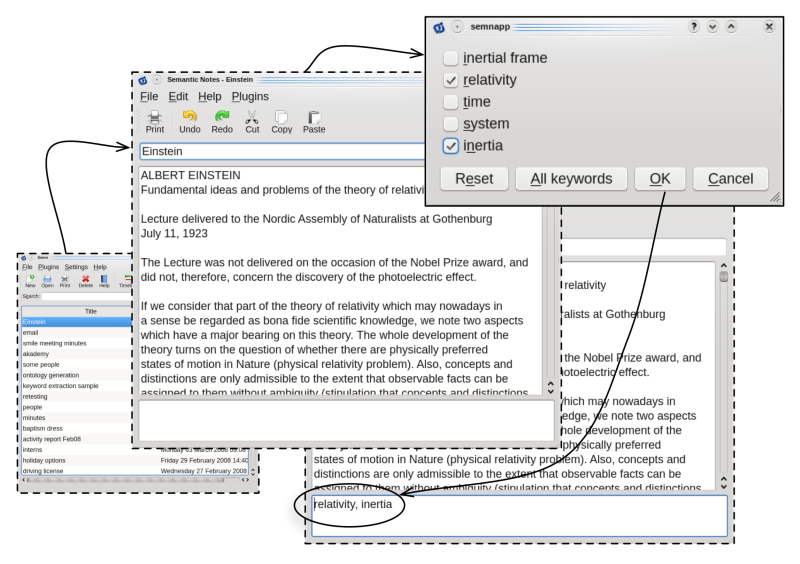
\includegraphics[width=\linewidth]{chapters/core/img/keywordextraction}
 \caption{User interface to keyphrase extraction in SemNotes.}
 \label{fig:keywordextraction}
\end{figure}

We have developed an extension to SemNotes, which uses the service to extract keyphrases from the text of the personal notes and suggest them to the user as tags. The text of personal notes can be small, thus adding difficulty to the extraction task. \cite{Schutz2008} details the way this challenge is tackled in the service. In SemNotes, the service can be called through the menu, and once the note is parsed the relevant terms found are presented to the user as tag suggestions. Figure \ref{fig:keywordextraction}, taken from \cite{Schutz2008}, shows a screenshot of the interface in an older version of SemNotes. If the user accepts any of the suggestions, they become tag resources and are stored in Nepomuk in the usual way.

\subsection{Controlled Language Extensions}

Controlled Natural Languages are well-defined subsets of a natural language with a restricted grammar and lexicon \cite{Schwitter2005}, in order to reduce ambiguity and complexity. In his Ph.D. thesis \cite{Davis2012PhD}, researches the use of Controlled Languages for ontology engineering and semantic annotation. We used SemNotes for prototype testing of both directions, while also providing a feasible use case for the services.

SemNotes, as a note-taking application, is well suited for Controlled Language use, since the main type of input from the users is textual. As a Semantic Desktop application it is also particularly well suited to ontology engineering due to the direct access provided by the framework to the underlying ontologies and desktop resources. As an annotation tool it is also a good testing ground for the semantic annotation using Controlled Language.

\subsubsection{Round Trip Ontology Authoring}

Controlled Natural Language proved efficient for creating ontologies in a user friendly way, for naive users who do not wish or do not need to learn how to use full-fledged ontology editors, nor want to dive into the complexities of ontology engineering. However simplified, Controlled Languages still require that the users be familiar with the vocabulary and syntax rules in order to use the language properly. The Round-trip Ontology Authoring environment described in \cite{Davis2008} aims to reduce the learning curve required to use Controlled Languages for ontology authoring. It combines and builds on the CLOnE controlled language for ontology editing \cite{Funk2007}, and Natural Language Generation from existing ontologies, to provide a simplified process: starting with an existing ontology, either imported or produced using CLOnE, generate the Controlled Language, edit the text, then parse it back into the modified ontology. Since the user only has to work with the textual representation of the ontology, we created a prototype extension for SemNotes to test the process.

Our extension allowed all the steps of the process --- import of existing ontologies, editing and exporting back into an ontology. It also had the added benefit of having access to all the ontologies loaded on the Semantic Desktop, and all the instances extracted from the personal data available on the desktop. Thus SemNotes allowed reuse of existing instances from the desktop in the ontology editing, and more importantly to create instances directly into the desktop repository, in a simple and user friendly way. It also meant that through this extension we could provide a way of easily creating or removing a relation between existing instances just by typing a sentence about it. 

\subsubsection{Controlled Language Annotation}

As we described before, SemNotes provides semi-automatic annotation of notes, by checking the available desktop resources and suggesting instances which are relevant to the note. Semi-automatic annotation is a mechanism often used to simplify the process of semantic annotation, and support the user. By employing Controlled Natural Language techniques, we can improve further the annotation process, in a user-friendly way. \cite{Davis2009} presents two approaches to applying Controlled Language to Semantic Annotation, called CLANN --- Controlled Language ANNotation. The two approaches were used to measure and evaluate the balance needed between expressiveness of the language and ease of use. CLANN is based on CLIE (Controlled Language for Information Extraction) and CLOnE. 

Semantic annotation with Controlled Language is better suited for some annotation scenarios than for others. CLANN is applied to two use cases, where the use of a controlled vocabulary is implicit --- meeting minutes and status reports. However, other possible use cases include the eHealth and business domains. The two use cases benefit from a semantic note-taking tool like SemNotes, thus creating an extension that uses CLANN was the next logical step.

The CLANN extension of SemNotes allows users to simultaneously create and annotate meeting minutes or status reports in Controlled Natural Language. It goes beyond the initial interlinking capabilities of SemNotes, by allowing the creation of different relations between the notes and desktop resources, as well as the creation of new resources and relations. CLANN uses a specially designed ontology for the meeting minutes and status reports, called MEMO, which is based on the desktop ontologies described in Section \ref{sub:nepomuk}. The notes must follow a specific template, which is then parsed by the service. In the parsing, the extension reuses SemNotes' mechanism for detecting related desktop resources. The information resulted from the parsed note is stored in the desktop repository.
